\section{Différenciation pour la symétrie}

\subsection{Activité des cocottes}\label{annexe:symetrie-act}

Énoncé initial : Chacune des cocottes blanches a été obtenue à partir de la grise par une transformation différente.  Classe les couples de cocottes en fonction des transformations utilisées pour les construire.

\begin{figure}[h!]
    \centering
    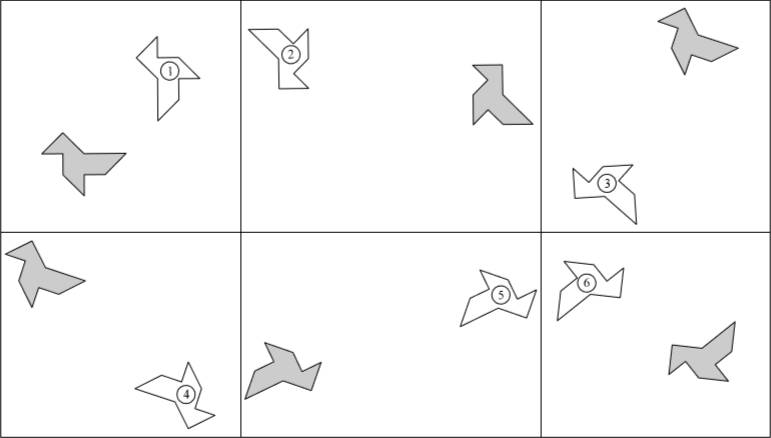
\includegraphics[width=0.9\linewidth]{img/activitemepcc.jpg}
    \caption{Source : \textit{Des maths ensemble et pour chacun 5\up{e}}}
    \label{fig:symetrie-act}
\end{figure}

\subsection{Fiches méthodologiques}\label{annexe:symetrie-fiches}

Les fiches méthodologiques sont scannées et présentes à cette adresse : \url{https://vvvictoire.github.io/memoire-meef/fiches-methodologiques.html}

\subsection{Activité en salle informatique}\label{annexe:symetrie-tice}

Pour cette séance, suite à plusieurs évaluations diagnostiques ponctuelles, j'avais décidé de retravailler la symétrie axiale et la symétrie centrale. L'objectif de cette séance est donc de leur permettre de consolider l'image mentale qu'ils se font des symétries en travaillant chez eux sur GeoGebra pendant les vacances. Pour cela, je leur ai préparé un exercice à réaliser seul sur GeoGebra pour se familiariser avec le logiciel et pour apprendre à s'auto-évaluer avant de refaire les activités seul à la maison.

Le fichier GeoGebra contient trois lettres dont les élèves devaient tracer le symétrique (par rapport à un point et par rapport à une droite). Dans un premier temps, ils devaient tracer le symétrique sur fond blanc et dans un deuxième temps en s'aidant du quadrillage. Enfin, ils devaient placer les axes de symétrie et les centres de symétrie de chaque lettre.

GeoGebra avait déjà été montré aux élèves comme un \textit{outil de conjecture}. Dans cette séance, c'est la première fois qu'ils utilisaient Gogebra en tant qu'\textit{outil de contrôle et de remédiation}. J'avais particulièrement insisté sur l'utilisation de l'outil \textit{Symétrie axiale} et de l'outil \textit{Symétrie centrale} comme \textbf{moyens de vérification} et non comme aides visuelles.

L'analyse complète de la séance, la fiche élève et le fichier GeoGebra associé sont disponibles à cette adresse : \url{https://vvvictoire.github.io/memoire-meef/extraits-de-portfolio.html}

\subsection{Analyse d'évaluation portant sur la symétrie}\label{annexe:symetrie-eval}

Dans un exercice de cette évaluation, les élèves devaient préciser la méthode employée pour construire le symétrique d'une ligne brisée connaissant l'emplacement d'un des segments du symétrique.

\begin{figure}[h!]
    \centering
    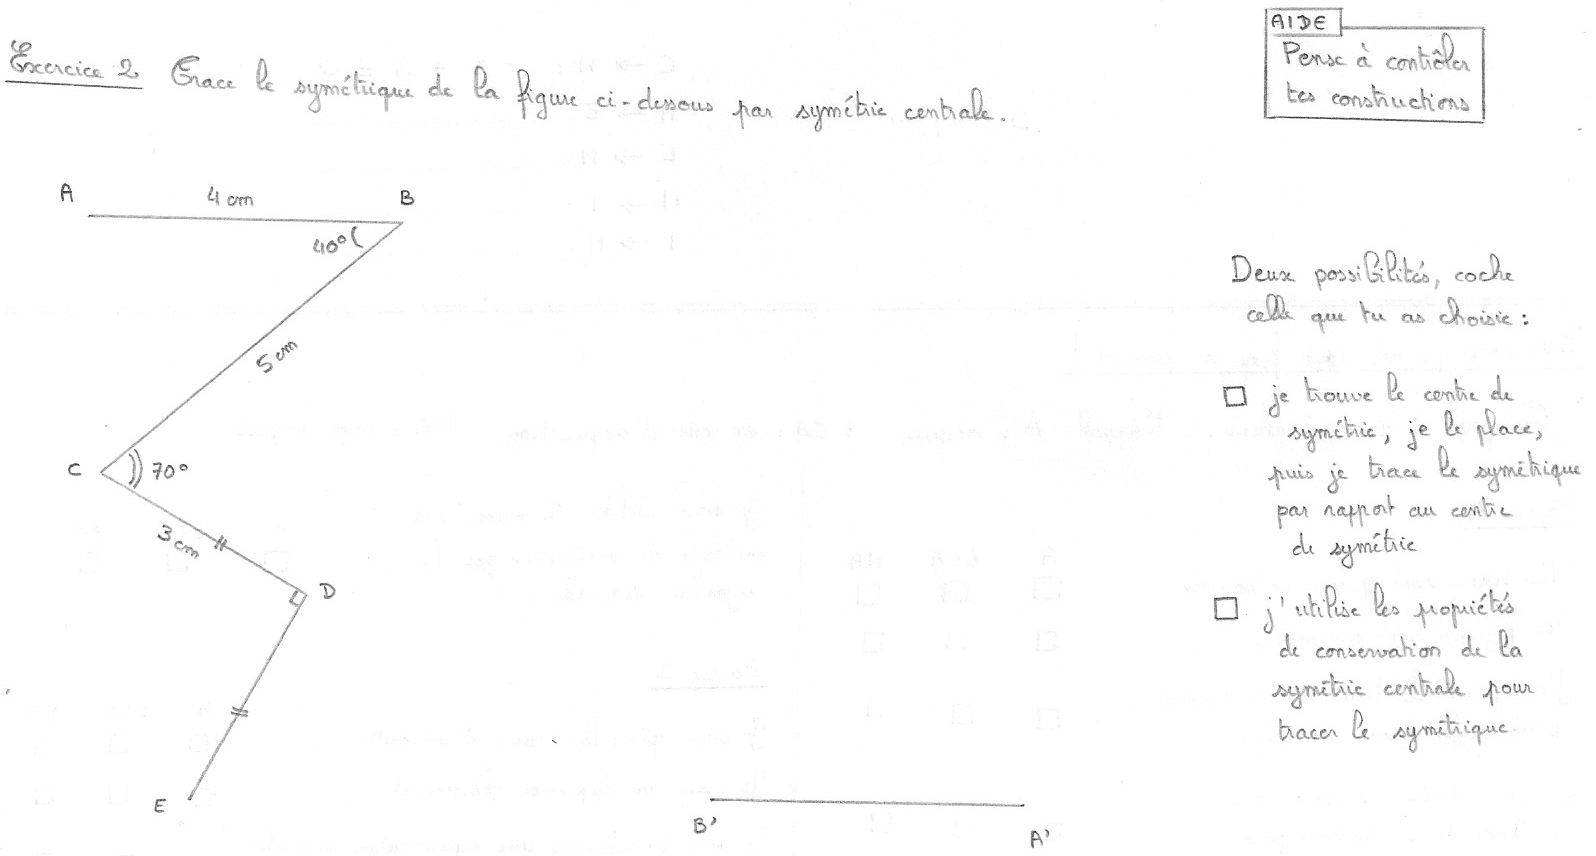
\includegraphics[width=\linewidth]{img/page1-exo2.png}
    \caption{Les propriétés de conservation de la symétrie centrale venaient d'être vues, peu d'élèves avaient eu le temps de se les approprier.}
    \label{fig:xav-eval}
\end{figure}

En dehors des évaluations à joker et des évaluations adaptées à un élève Italien en difficulté avec la langue française, ceci est la seule question différenciée proposée dans toutes mes évaluations. Cela n'est pas clairement précisé dans l'analyse de cette évaluation, mais il est important de préciser que cette question n'apportait pas de point pour la note chiffrée, bien qu'elle apparaisse dans la grille d'évaluation par compétences.

L'analyse complète de l'évaluation est disponible à cette adresse : \url{https://vvvictoire.github.io/memoire-meef/extraits-de-portfolio.html}

\clearpage

\section{Différenciation pour les angles alternes-internes}

\subsection{Évaluations diagnostiques}\label{annexe:angles-prod1}

Voici quelques citations extraites de copies d'élèves. La question initiale était : \og Quelle est la définition d'un angle alterne-interne ? \fg{}
\begin{itemize}
\item Deux droites parallèles coupées par une droite sécante [donnent des angles] alternes internes de même mesure (confusion entre définition et propriété)
\item Alterne : angle à l'extérieur de la droite qui coupe les deux droites parallèles. Interne : angle à l'intérieur de la droite qui coupe les deux droites parallèles.
\item Quand il y a deux droites parallèles coupées par une droite sécante, les deux angles sont à l'intérieur et disposés de part et d'autre de la sécante.
\item C[e sont] deux droites parallèles qui sont tranchées par une autre droite.
\end{itemize}

Sur nombre de copies, les élèves ont répondu à la deuxième question (\og Dessinez une figure où vous indiquerez les deux paires d'angles alternes-internes \fg{}) par un schéma comportant deux droites parallèles (bien qu'aucun élève ne précise explicitement que les droites sont parallèles). Un seul élève a tracé des droites non parallèles et un élève a produit ceci :

\begin{figure}[h!]
    \centering
    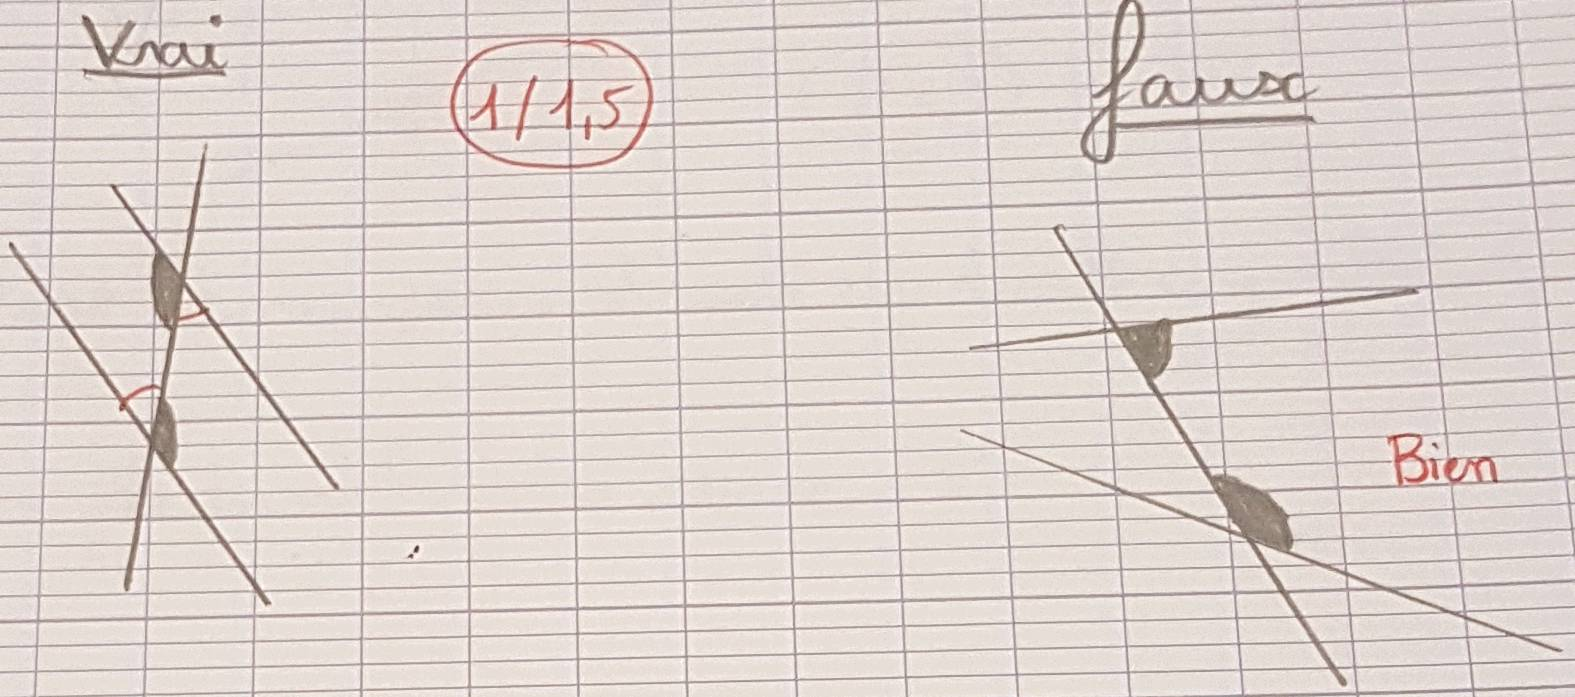
\includegraphics[width=0.6\linewidth]{img/anglesquestion.jpg}
    \caption{Associe-t-il la condition de droites parallèles à la définition des angles alternes-internes ou est-ce un hasard ?}
\end{figure}

Les captures d'écran associées à ces citations sont consultables à cette adresse : \url{https://vvvictoire.github.io/memoire-meef/angles-productions-d-eleves.html}

\clearpage

\subsection{Fiches d'exercice}\label{annexe:angles-fiches}

\begin{figure}[h!]
    \centering
    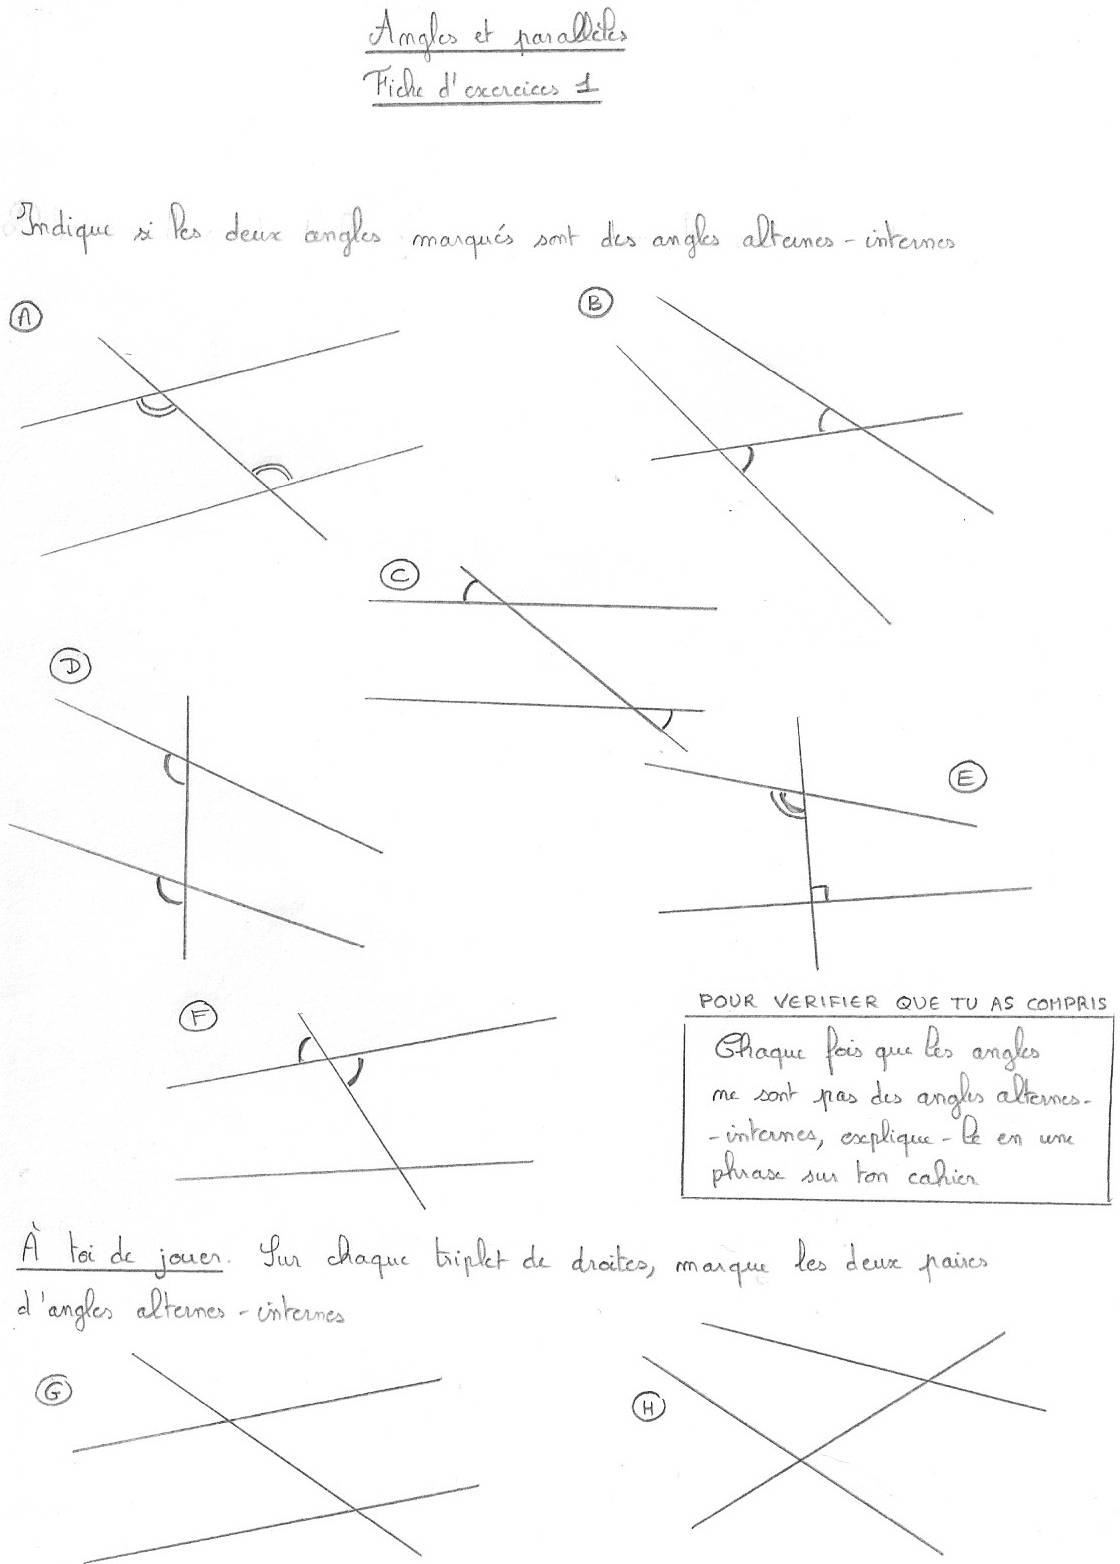
\includegraphics[width=0.6\linewidth]{img/anglesfiche1.jpg}
    \caption{Reconnaissance d'angles alternes-internes (cette feuille a fait l'objet d'une évaluation diagnostique). L'exercice supplémentaire n'a pas été traité.}
    \label{fig:angles-fiche1}
\end{figure}

\begin{figure}[h!]
    \centering
    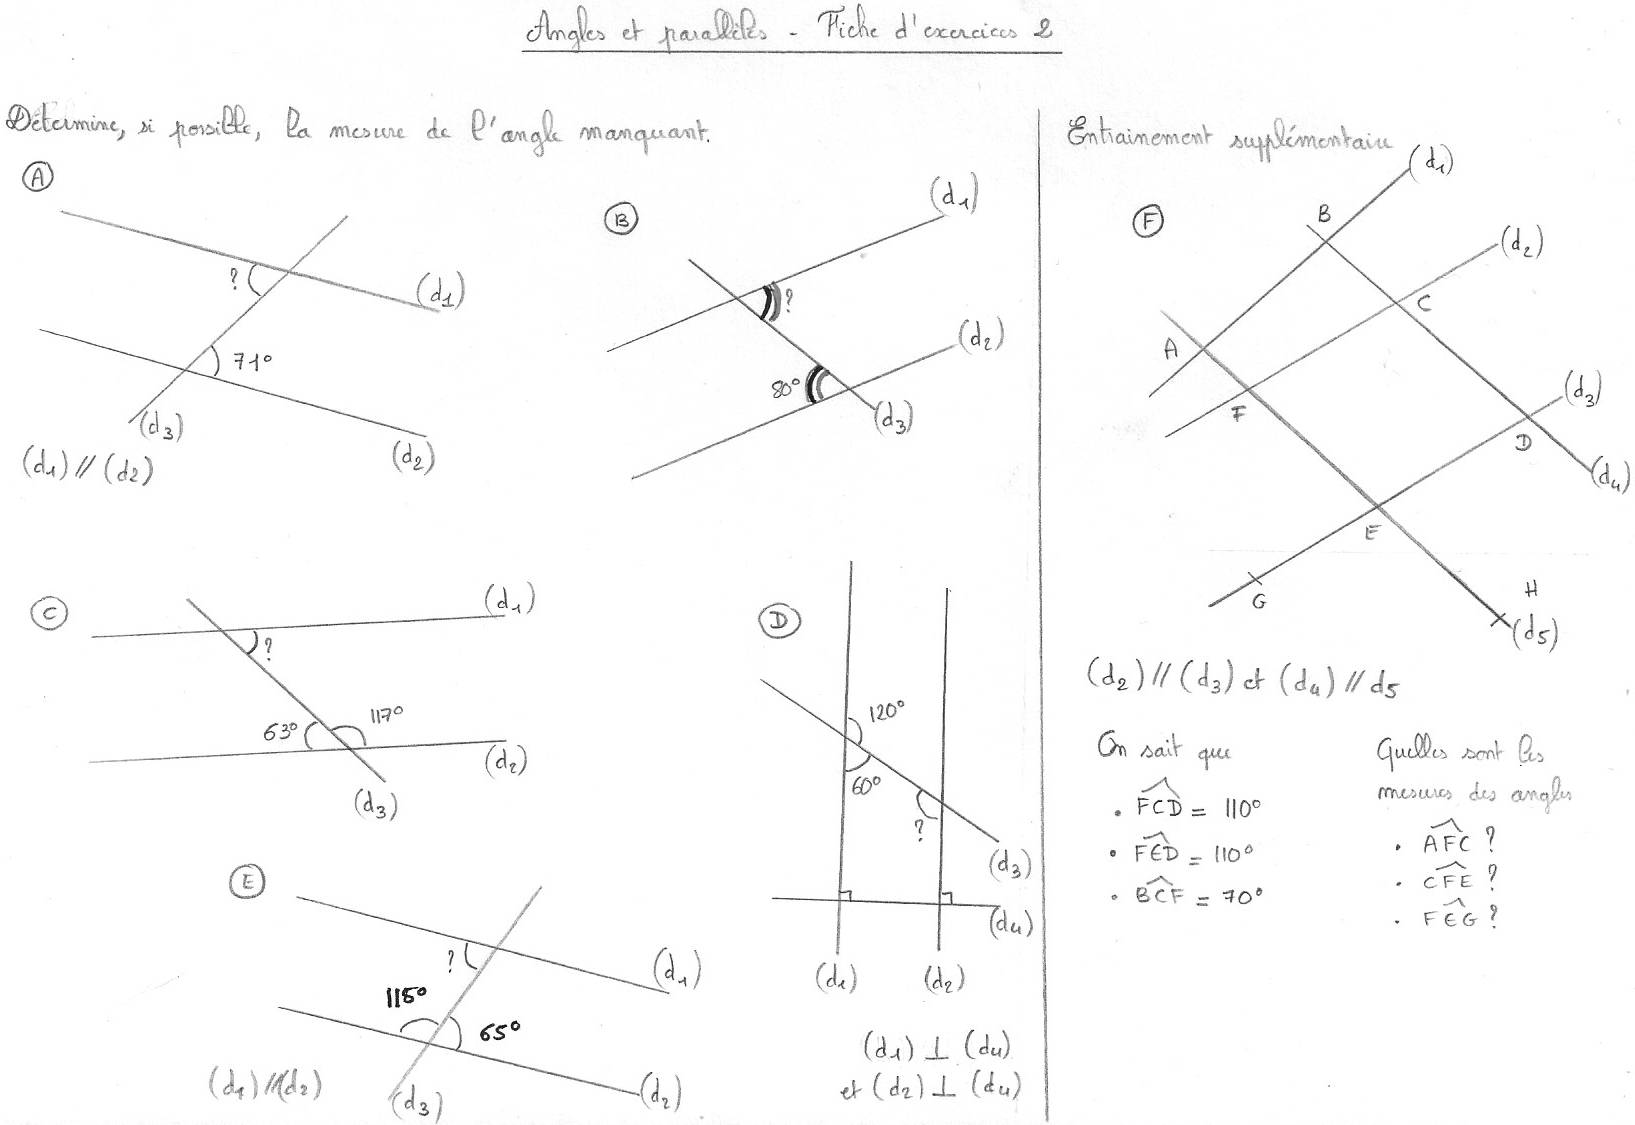
\includegraphics[width=0.8\linewidth]{img/anglesfiche2.jpg}
    \caption{Détermination de la valeur de l'angle par application directe de la propriété. Difficulté liée à la géométrie abstraite : les élèves doivent tenir compte des codages. Un exercice supplémentaire pour les élèves en avance.}
    \label{fig:angles-fiche2}
\end{figure}

\begin{figure}[h!]
    \centering
    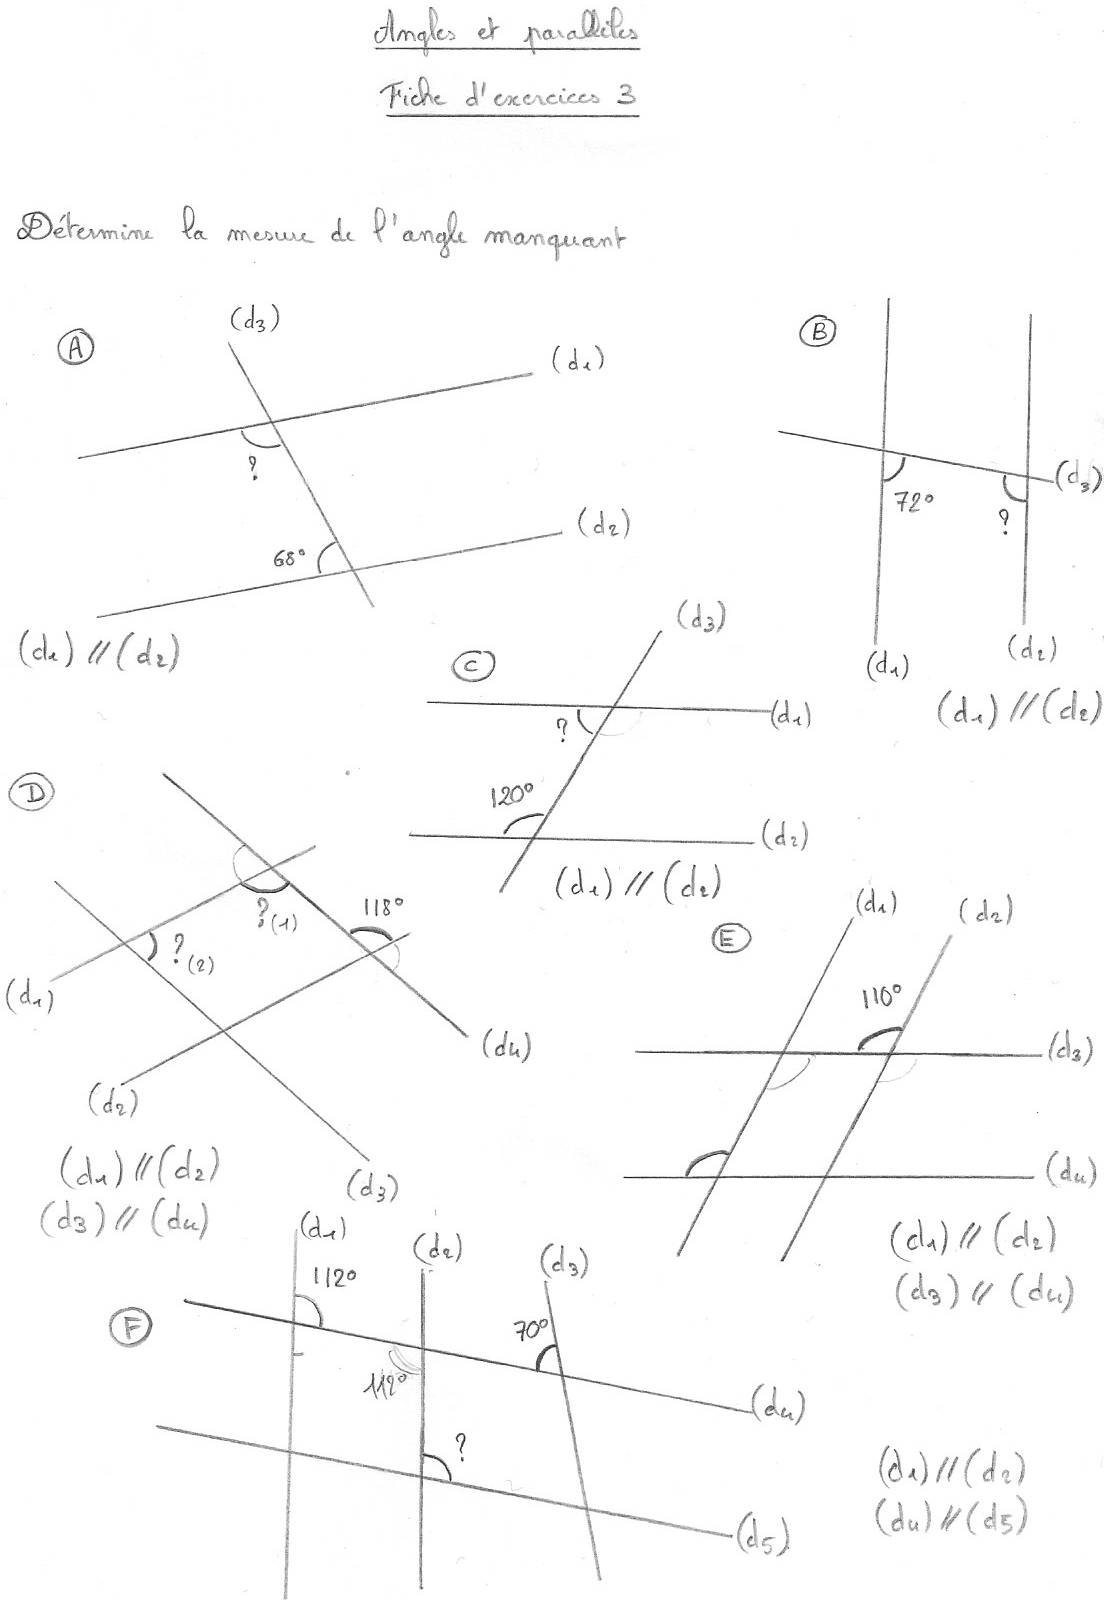
\includegraphics[width=0.6\linewidth]{img/anglesfiche3.jpg}
    \caption{Détermination de la valeur de l'angle soit par application directe de la propriété, soit par calcul du supplémentaire. Les schémas D, E et F étaient réservés aux élèves en avance.}
    \label{fig:angles-fiche3}
\end{figure}

\clearpage

\subsection{Histoire de la coccinelle et de la libellule}\label{annexe:angles-prod2}

\begin{figure}[h!]
    \centering
    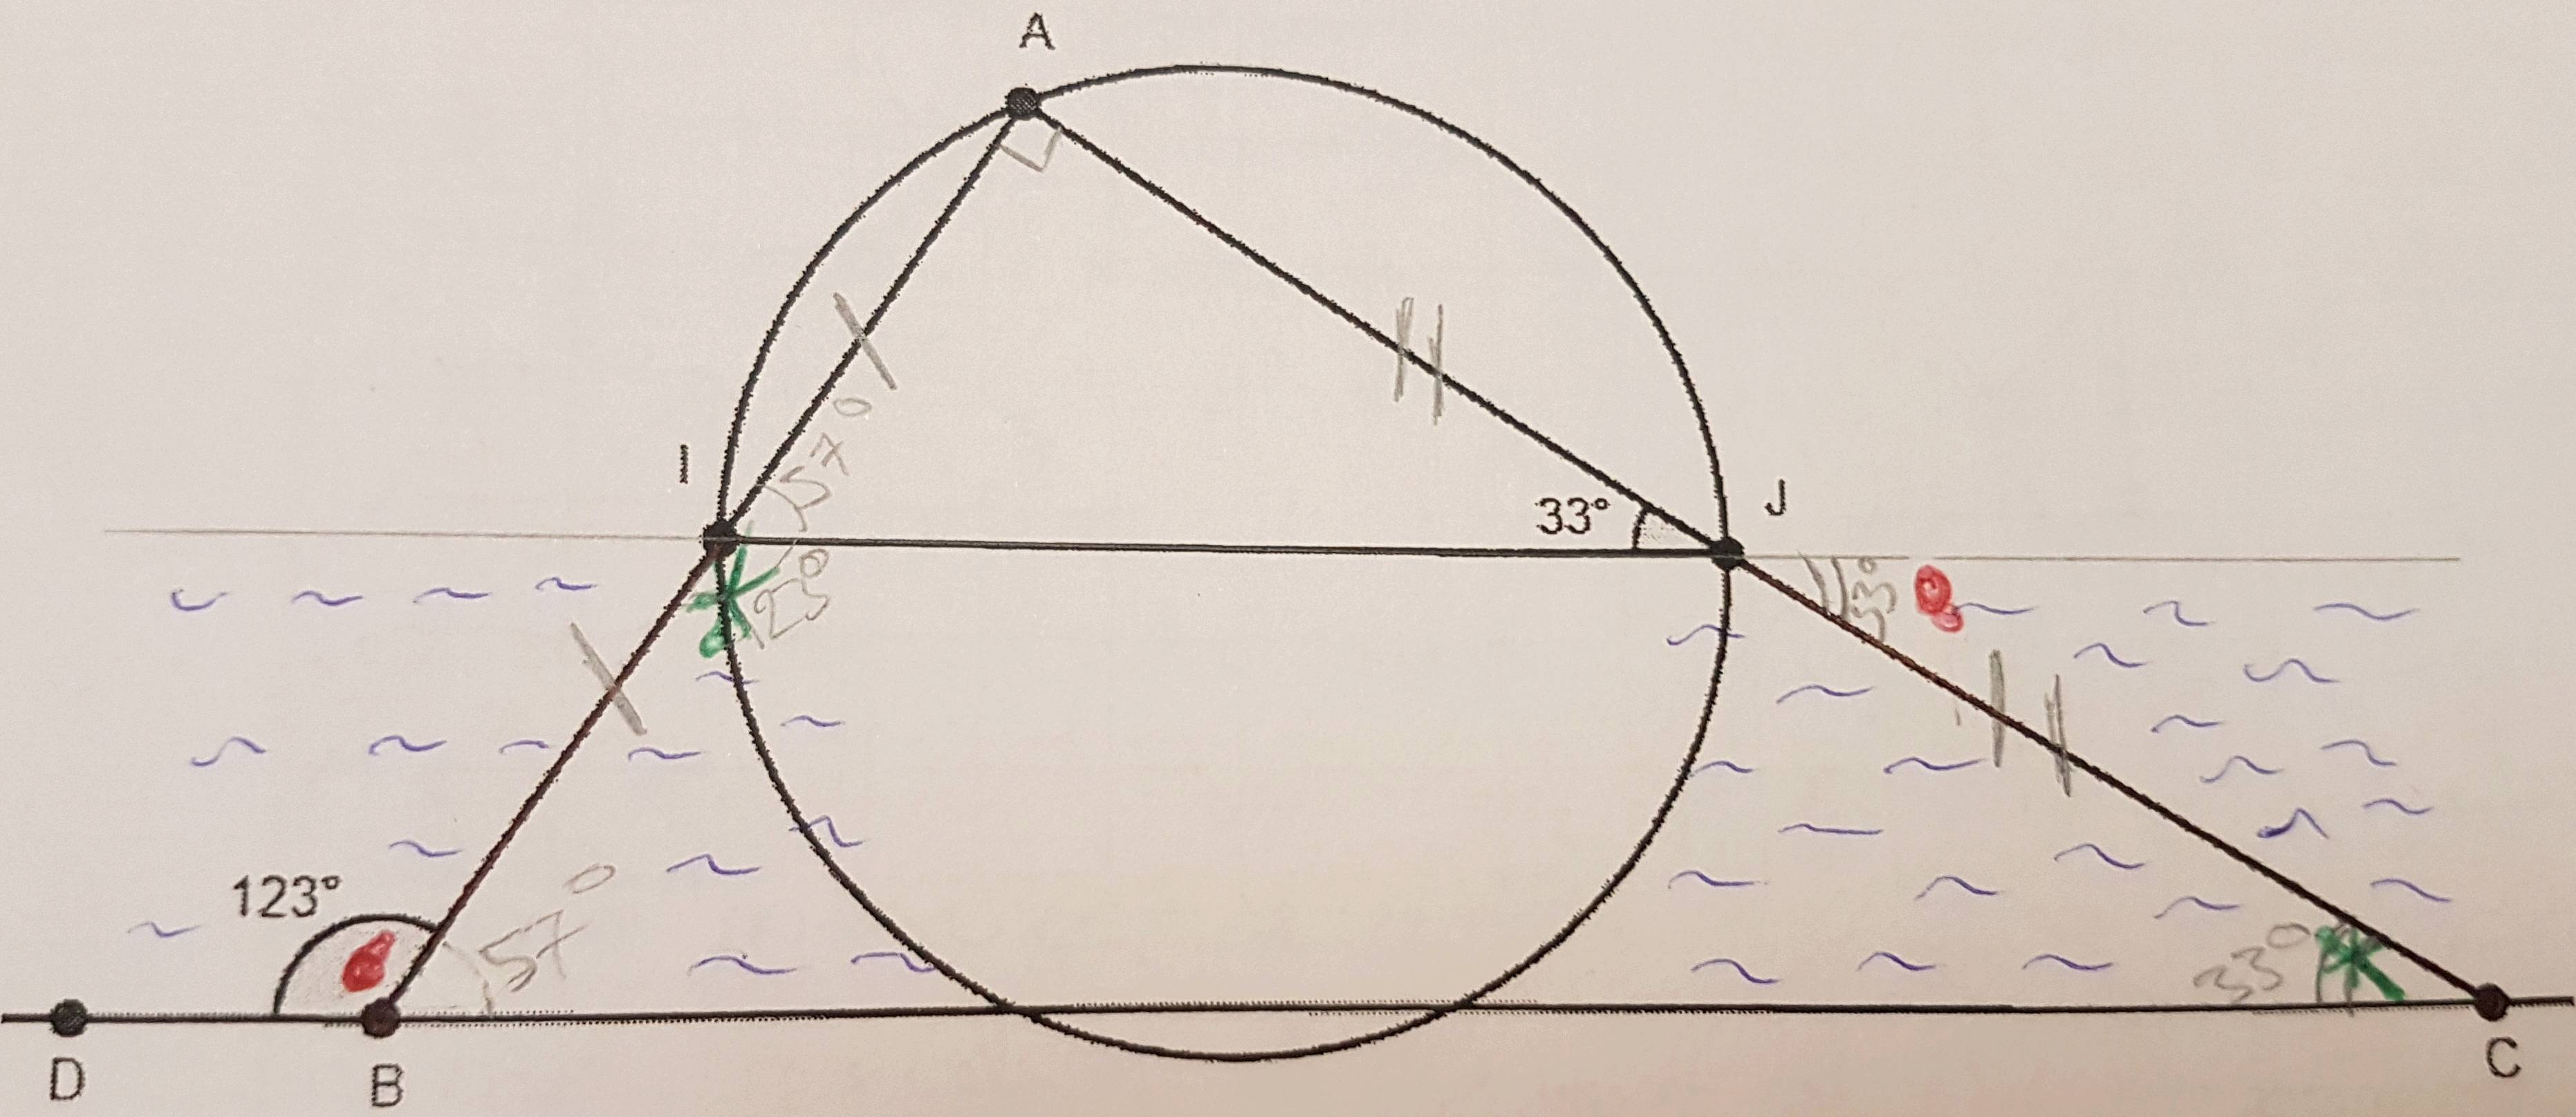
\includegraphics[width=\linewidth]{img/insectes-point.jpg}
    \caption{Une version où la coccinelle et la libellule sont dessinées.}
    \label{fig:angles-insecte1}
\end{figure}

\begin{figure}[h!]
    \centering
    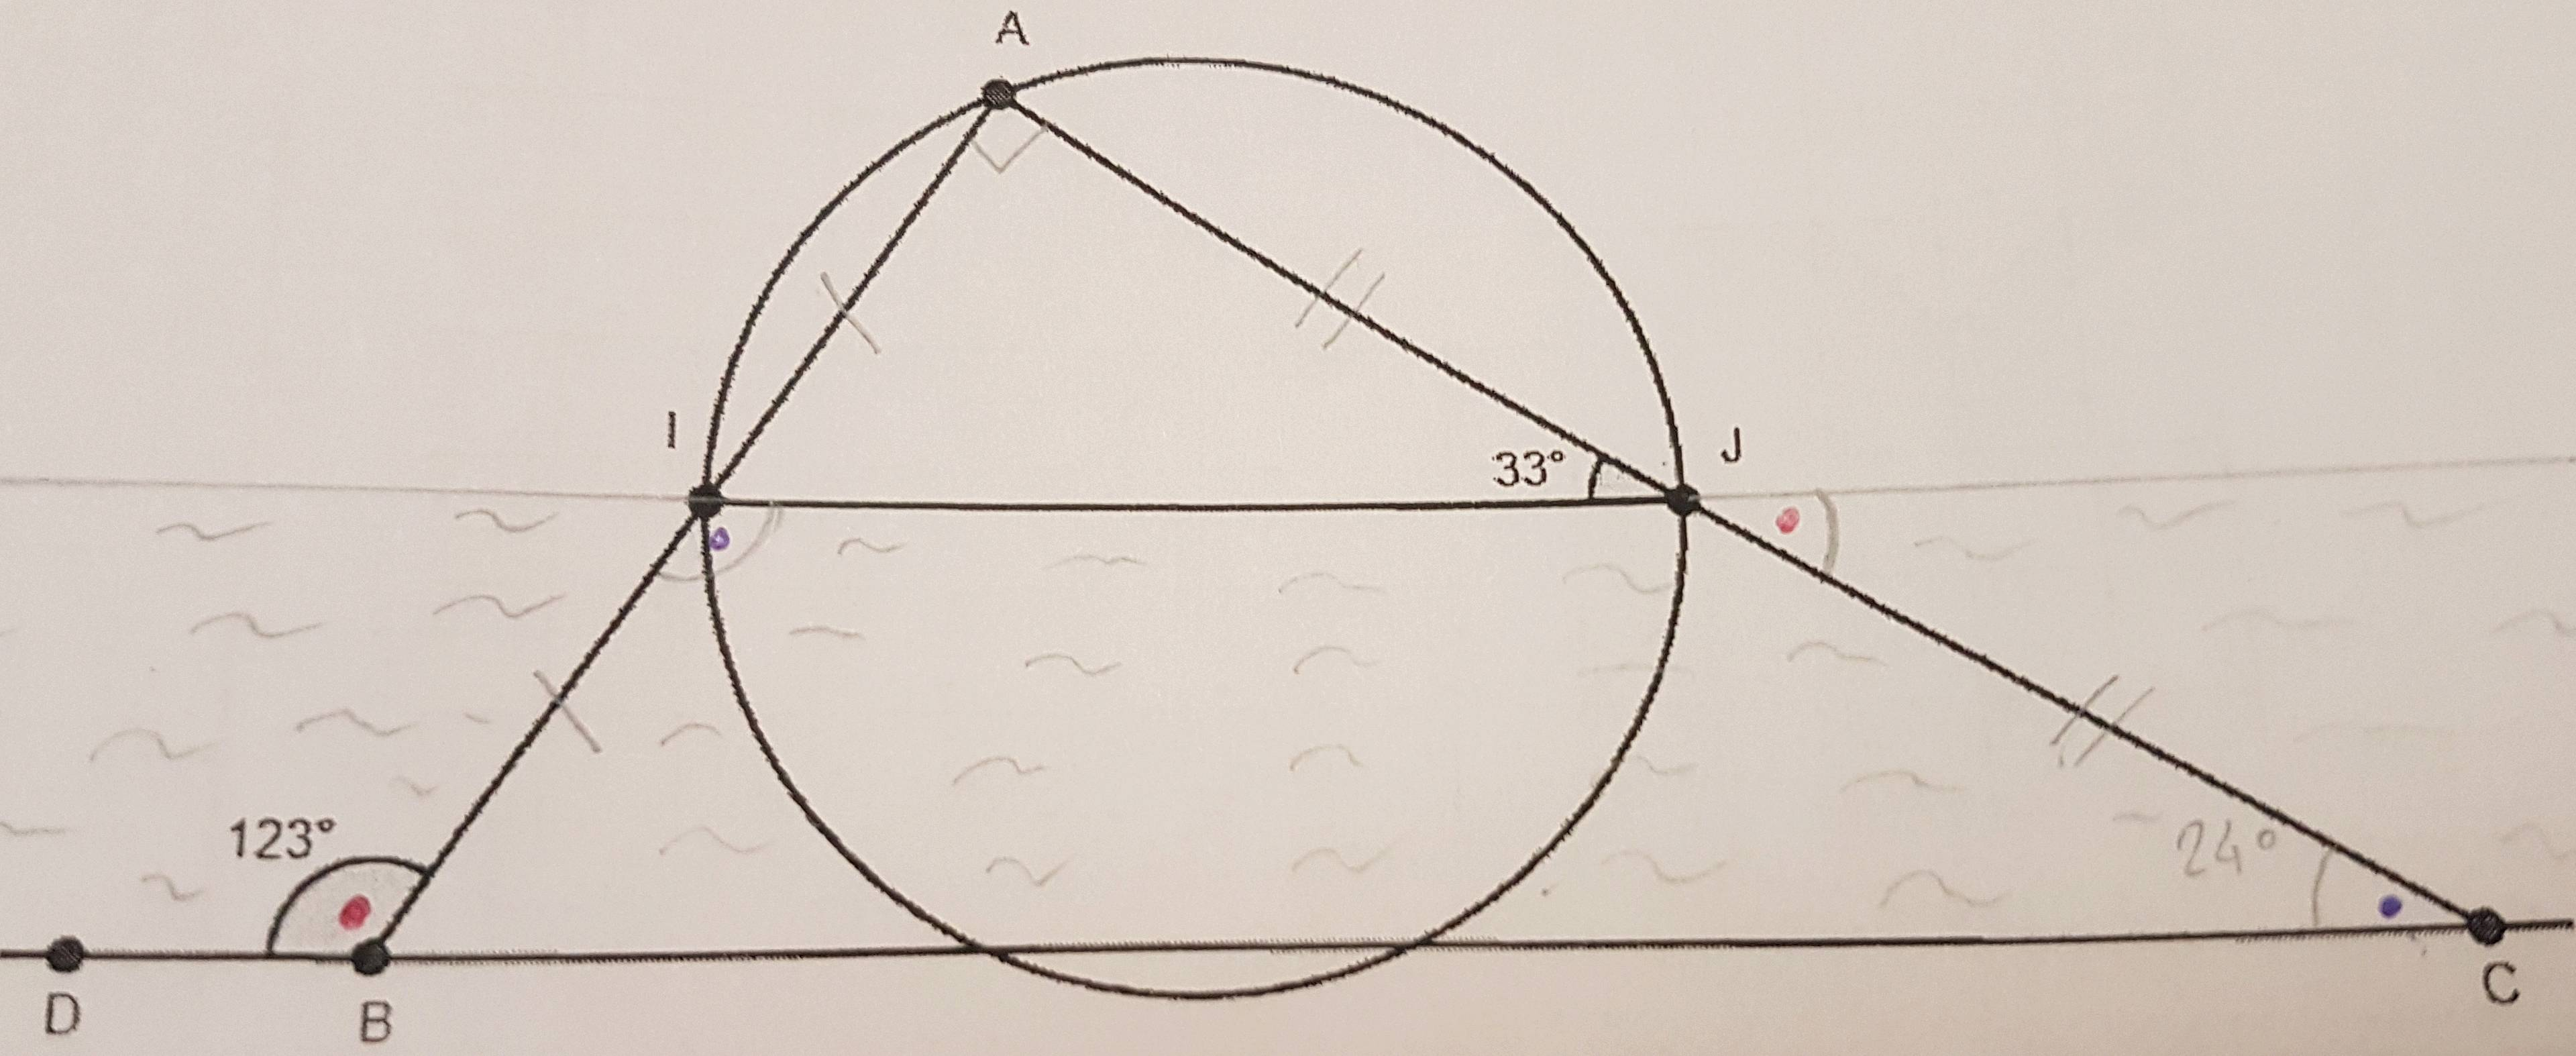
\includegraphics[width=\linewidth]{img/insectes.jpg}
    \caption{Une version évoluée où la coccinelle et la libellule sont schématisées par des points.}
    \label{fig:angles-insecte2}
\end{figure}
